\documentclass[10pt]{article}
\usepackage[letterpaper,margin=1in]{geometry}
\usepackage[T1]{fontenc}
\usepackage{mathptmx}
\usepackage[scaled=0.92]{helvet}
\usepackage{courier}
\usepackage[numbers,sort&compress]{natbib}
\usepackage{graphicx,booktabs,microtype,xcolor,amsmath,amssymb}
\usepackage{tikz}
\usetikzlibrary{arrows.meta,positioning,calc,fit,decorations.pathreplacing}
\usepackage[colorlinks=true,linkcolor=blue!50!black,citecolor=blue!50!black,urlcolor=blue!50!black]{hyperref}
\usepackage[capitalize,noabbrev]{cleveref}
\definecolor{tsix}{HTML}{1F5FA8}
\setlength{\parskip}{2pt}
\renewcommand{\floatpagefraction}{0.8}

\title{\textbf{T16: A Decode-Cost-Driven Trellis Format for Running a 552B\\Mixture of Experts on Two Consumer GPUs}}
\author{Aleksey Smolenchuk\\\texttt{lxe@lxe.co}\\[2pt]\small dsx project, \url{https://github.com/lxe/dsx}}
\date{October 2026}

\begin{document}
\maketitle

\begin{abstract}
DeepSeek-V4.1-Flash-1017 is a 552B-parameter mixture of experts, and 98.5\% of its weights are 15{,}360 routed
experts. To run it on a desktop with two 24\,GB RTX 3090s and 128\,GB of RAM, those experts must take about 1.9 bits
per weight. They must also decode fast in two very different places: as single-token GEMVs on the GPUs, and as AVX-VNNI
loops on the CPU for the roughly 12{,}600 experts that live in RAM.
We present T16, an expert format built from a measured decode-cost model of both processors. T16 keeps the bitshift
trellis of QTIP and ExLlamaV3 but replaces its codebook. A weight's value comes from one 16-bit multiply and a
two-byte sum, which makes dequantization and the dot product one fused integer operation on both processors, at 4\%
more mean squared error than ExLlamaV3's codebook on Gaussian data. Positions inside each tile are column-major, which
costs no measurable quality and lets one file feed fast row-walking kernels.
On the quantizer side we contribute a dense fractional-bit Viterbi kernel that is bit-identical to ExLlamaV3's and
5.1$\times$ faster at 1.5 bits. We also identify a systematic output shrinkage of MSE-optimal trellis reconstructions
(the plain gain is $1-\text{relative MSE}$) and correct it for free in the stored output scales; on a half-T16 model
this took KL divergence from 0.31 to 0.25. With experts at 1.5--2.5 bits, the full model scores KL 0.194 against the
FP8 model on the Lucebox evaluation, 28\% lower than the same-size build with Unsloth's UD-IQ1\_M experts (0.272).
Its expert kernels are 20--34\% faster on the CPU and 22\% faster on the GPU than that build's, and it decodes at
34.9 tokens/s on the two RTX 3090s. Quantizing all 15{,}360 experts took 6.1 hours on one rented GPU for \$16.
\end{abstract}

\section{Introduction}

Large mixture-of-experts (MoE) models put most of their weights in experts that each token uses only rarely.
DeepSeek-V4.1-Flash-1017~\cite{dsv41} (hereafter \emph{V4.1}) has 40 MoE layers with 384 routed experts each, plus one
shared expert. A router picks 6 routed experts per token per layer. Each routed expert is a SwiGLU block with three
matrices: gate and up ($2304 \times 5120$) and down ($5120 \times 2304$). Together the routed experts hold
$40 \cdot 384 \cdot 3 \cdot 5120 \cdot 2304 = 543.6$B of the model's 552B weights. The model also carries a 196B
Engram memory, a table of $n$-gram embeddings read by lookup rather than matrix multiply. We leave that table at 4--6
bits and do not discuss it further.

dsx~\cite{dsx} is an inference engine written for this one model and one class of machine: two 24\,GB GPUs, 128\,GB of
RAM and an NVMe drive. \Cref{fig:system} shows how it uses that machine. The dense half of the network and the hottest
experts run on the GPUs, about 12{,}600 experts live in a RAM arena where the CPU computes them in place, and the
coldest are read from the file. Each token touches 240 expert calls (6 per layer), about 2\,GB of expert weights at the
bit widths used here. About 74\% of expert picks are served from VRAM, and the CPU's share sets decode speed.

This placement fixes what the expert format must do. It must reach about 1.9 bits per weight to fit, and at that rate
it must keep quality close to the FP8 original. Most importantly, it must decode at memory speed on \emph{both}
processors, because the same file is read by GPU kernels for resident experts and by CPU kernels for the arena. Existing
formats fall short on one side or the other. llama.cpp's IQ codebooks~\cite{llamacpp}, as mixed by Unsloth's UD
builds~\cite{unsloth}, decode reasonably on both but trail trellis codes in accuracy. ExLlamaV3's trellis
codes~\cite{exllamav3,qtip} come close to the Gaussian rate-distortion bound, but ExLlamaV3 keeps every weight in VRAM,
and its codebook costs a 32-bit multiply per weight, which desktop CPUs execute slowly.

\paragraph{Contributions.}
\begin{itemize}\setlength{\itemsep}{1pt}
\item A decode-cost model for single-token expert GEMVs on an RTX 3090 and an i7-12700K, built from measured
per-instruction throughputs, and the per-weight instruction budget it implies at 1.5--2.5 bits (\cref{sec:cost}).
\item \textbf{T16}, a trellis codebook chosen under that budget: a 16-bit multiply and a two-byte sum, which fuse with
the activation dot product into \texttt{vpdpbusd} on the CPU and \texttt{dp4a} on the GPU. We pair it with
column-major tile positions, which cost no quality. T16 kernels beat every IQ format of UD's mix on both processors
(\cref{sec:format}).
\item A dense fractional-bit Viterbi kernel for ExLlamaV3's quantizer: bit-identical output, 5.1$\times$ faster at
1.5 bits, and full-model quantization 2.1$\times$ cheaper (\cref{sec:quantizer}).
\item An analysis of the output shrinkage of MSE-optimal trellis reconstructions, and a free correction in the stored
output scales (\cref{sec:gain}).
\item A routing-aware calibration set for a 384-expert MoE: the model's own reasoning, scrubbed coding-agent
transcripts and public agent trajectories, topped up with probe sequences until rare experts get enough tokens
(\cref{sec:calib}).
\item End-to-end results for a 552B model on two RTX 3090s, with quality, speed and quantization cost
(\cref{sec:results}).
\end{itemize}

\begin{figure}[t]
\centering
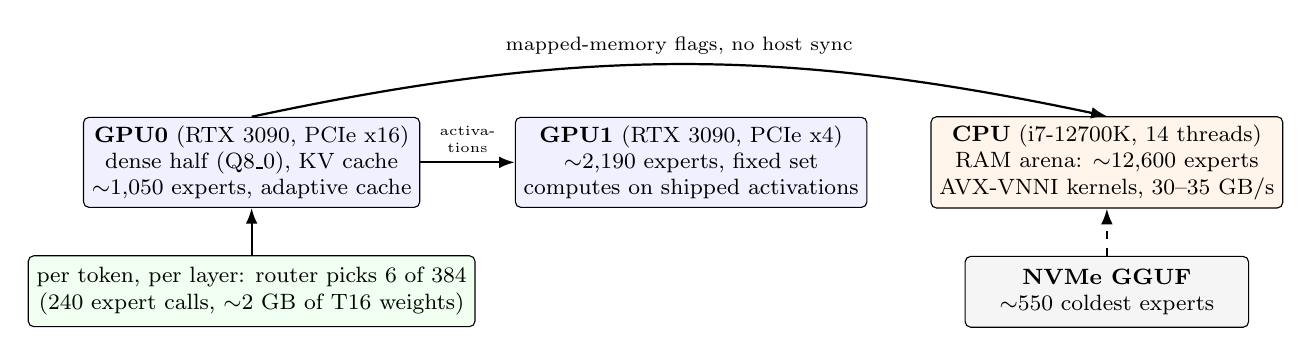
\begin{tikzpicture}[font=\footnotesize, box/.style={draw, rounded corners=2pt, align=center, minimum height=9mm, inner sep=3pt},
  arr/.style={-{Latex[length=2mm]}, thick}]
\node[box, fill=blue!6, minimum width=36mm] (g0) {\textbf{GPU0} (RTX 3090, PCIe x16)\\dense half (Q8\_0), KV cache\\$\sim$1{,}050 experts, adaptive cache};
\node[box, fill=blue!6, minimum width=36mm, right=12mm of g0] (g1) {\textbf{GPU1} (RTX 3090, PCIe x4)\\$\sim$2{,}190 experts, fixed set\\computes on shipped activations};
\node[box, fill=orange!8, minimum width=36mm, right=8mm of g1] (cpu) {\textbf{CPU} (i7-12700K, 14 threads)\\RAM arena: $\sim$12{,}600 experts\\AVX-VNNI kernels, 30--35 GB/s};
\node[box, fill=gray!8, below=6mm of cpu, minimum width=36mm] (disk) {\textbf{NVMe GGUF}\\$\sim$550 coldest experts};
\node[box, fill=green!6, below=6mm of g0, minimum width=36mm] (tok) {per token, per layer: router picks 6 of 384\\(240 expert calls, $\sim$2 GB of T16 weights)};
\draw[arr] (tok.north) -- (g0.south);
\draw[arr] (g0.east) -- node[above, font=\tiny, align=center]{activa-\\tions} (g1.west);
\draw[arr] (g0.north) to[bend left=12] node[above, font=\scriptsize]{mapped-memory flags, no host sync} (cpu.north);
\draw[arr, dashed] (disk.north) -- (cpu.south);
\end{tikzpicture}
\caption{Where V4.1's 15{,}360 routed experts are computed during decode in dsx on 2$\times$RTX 3090 + 128\,GB RAM.
The expert format is read by GPU kernels (resident experts) and CPU kernels (the arena), so it has to decode fast on
both.}
\label{fig:system}
\end{figure}

\section{Background and related work}
\label{sec:related}

\paragraph{Weight-only post-training quantization.}
GPTQ~\cite{gptq} rounds weights one input column at a time, feeding each column's error forward through the inverse of
the input Hessian $H = \mathbb{E}[x x^\top]$. QuIP~\cite{quip} recast this as LDLQ, rounding with the LDL factor of
$H$, and introduced \emph{incoherence processing}: random orthogonal transforms that make weights near Gaussian and
spread outliers. QuIP\#~\cite{quipsharp} used fast randomized Hadamard transforms and an 8-dimensional $E_8$ lattice
codebook (E8P). QuaRot~\cite{quarot} rotates activations in the same spirit. Vector and additive codebooks (AQLM, VPTQ,
PV-Tuning)~\cite{aqlm,vptq,pvtuning} reach 2 bits with large learned codebooks, at substantial encoding cost.
HIGGS~\cite{higgs} uses data-free Gaussian-optimal grids after Hadamard rotation. GSQ~\cite{gsq} learns scalar
assignments with Gumbel-softmax sampling.

\paragraph{Trellis-coded quantization.}
Trellis-coded quantization (TCQ)~\cite{tcq} quantizes a whole sequence jointly with the Viterbi
algorithm~\cite{viterbi}. QTIP~\cite{qtip} made TCQ practical for LLMs with a \emph{bitshift} trellis. Each weight's
codeword index is a sliding $L$-bit window over a bit stream that advances $K$ bits per weight, so decoding is
parallel. The codebook is computed from the window by a few integer instructions (1MAD, 3INST) or a small table (HYB),
and QTIP reports Gaussian MSE within about 10\% of the rate-distortion bound at 2 bits. ExLlamaV3 (EXL3)~\cite{exllamav3}
is a streamlined QTIP: 16$\times$16 tiles with $L = 16$, 128-wide Hadamard transforms on both sides with per-channel
scales, LDLQ over 16-row bands, and half-integer rates. Its default codebook (\texttt{mul1}) multiplies the window by a
32-bit constant and sums the product's four bytes. Q-Palette~\cite{qpalette} and YAQA~\cite{yaqa} extend QTIP with
fractional rates, mixed schemes and Hessians of the full-model KL. XOR-Trellis~\cite{xortrellis} drops the Hadamard in
favor of curvature-aware palettes. ik\_llama.cpp's IQ*\_KT types~\cite{iklamacpp} code independent 8-weight groups from
16-bit seeds without a Viterbi search. Our work keeps EXL3's quantizer and replaces the codebook. The choice is driven
by measured decode cost on desktop hardware rather than by MSE alone.

\paragraph{Running MoE models on consumer hardware.}
llama.cpp~\cite{llamacpp} offloads experts to the CPU with its ggml backend, and its IQ formats (8-weight codebook
entries from global tables) underlie Unsloth's per-tensor ``dynamic'' mixes~\cite{unsloth}. KTransformers~\cite{ktransformers}
splits MoE inference across CPU and GPU. dsx~\cite{dsx} places experts by measured routing frequency across GPUs and a
RAM arena, with no host synchronization inside a token. Its first builds used scalar ternary, 2-bit and 3-bit tiers from
the Xolotl pipeline~\cite{xolotl} and reached KL 0.373 at 148\,GB. Unsloth's UD-IQ1\_M experts did markedly better at
the same size (KL 0.272), and our analysis traced much of the difference to how well they transfer from calibration
text to new text. That observation
motivated T16.

\section{A decode-cost model for expert GEMVs}
\label{sec:cost}

In decode, each expert matrix multiplies one activation vector, so its runtime is the larger of the time to read its
bytes and the time to execute its per-weight instructions on the busiest execution pipe. We measured both sides on the
target machine. GPU throughput was measured with one 1024-thread block per SM and \texttt{clock64}. CPU throughput was
measured per core clock with eight independent dependency chains, calibrated by a dependent add chain
(\cref{tab:isa}).

\begin{table}[t]
\centering\small
\begin{tabular}{@{}llr@{\hspace{2em}}llr@{}}
\toprule
\multicolumn{3}{c}{RTX 3090 (82 SMs, $\sim$1.74 GHz at 285 W), lanes / clock / SM} & \multicolumn{3}{c}{i7-12700K P-core, instructions / clock} \\
\cmidrule(r){1-3}\cmidrule(l){4-6}
SHF, LOP3, PRMT & ALU & 64 & \texttt{vpshufb}, \texttt{vpsrld} & & 2 \\
IMAD, IDP4A, HFMA2 & FMA-heavy & 64 & \texttt{vpmullw} (16-bit) & & 1.6 \\
FFMA & FMA & 128 & \texttt{vpdpbusd} (AVX-VNNI) & & 1.6 \\
LDS, data-dependent index & shared & 16 & \texttt{vpmulld} (32-bit) & & 0.74 \\
int8 \texttt{mma} m16n8k32 & tensor & 0.2 / clk & \texttt{vpgatherdd} (8 dwords) & & 0.17 \\
\bottomrule
\end{tabular}
\caption{Measured instruction throughput (\texttt{bench/gpu\_isa.cu}, \texttt{bench/cpu\_isa.c}). E-cores run the
vector instructions about 4$\times$ slower and add little.}
\label{tab:isa}
\end{table}

\paragraph{Budget.}
At $\sim$850\,GB/s the GPU streams 3.4 trillion 2-bit weights per second. Matching that with 82 SMs leaves about 2.2
instructions per weight on each of the ALU and FMA-heavy pipes (1.6 at 1.5 bits, 2.7 at 2.5 bits) before decode, not
memory, sets the time. The CPU's 43\,GB/s across eight P-cores leaves about 4.5 weights per core clock at 2 bits.
Two consequences follow. First, a data-dependent table lookup costs the GPU four ALU instructions' worth of throughput,
and a gather yields only 1.4 entries per clock on a P-core, so a lookup code pays only if one lookup yields at least
four weights. Second, a 32-bit multiply per weight (EXL3's \texttt{mul1}) runs at 0.74 per clock on the CPU, which by
itself limits a core to below the RAM rate.

\paragraph{The floor.}
A bitshift trellis needs at least one window extraction (a funnel shift), one codebook evaluation and its share of the
dot product per weight. If the codebook value is affine in a sum of bytes of an integer product, the dot product
becomes exact integer arithmetic,
\begin{equation}
\sum_w f(s_w)\, x_w \;=\; \alpha \Big(\sum_w \textstyle\sum_{\text{bytes } j} p_{w,j}\, x_w\Big) + \beta \sum_w x_w,
\qquad p_w = (s_w \cdot M) \bmod 2^{16},
\label{eq:fused}
\end{equation}
which \texttt{vpdpbusd} (CPU) and \texttt{dp4a} (GPU) evaluate directly on the product bytes and int8 activations. With
two consecutive rows' products packed by one PRMT and dot-multiplied with $[x_k\, x_k\, x_{k+1}\, x_{k+1}]$, the GPU cost
is 1.5 ALU plus 1.5 FMA-heavy instructions per weight, inside the budget.

\section{The T16 format}
\label{sec:format}

\begin{figure}[t]
\centering
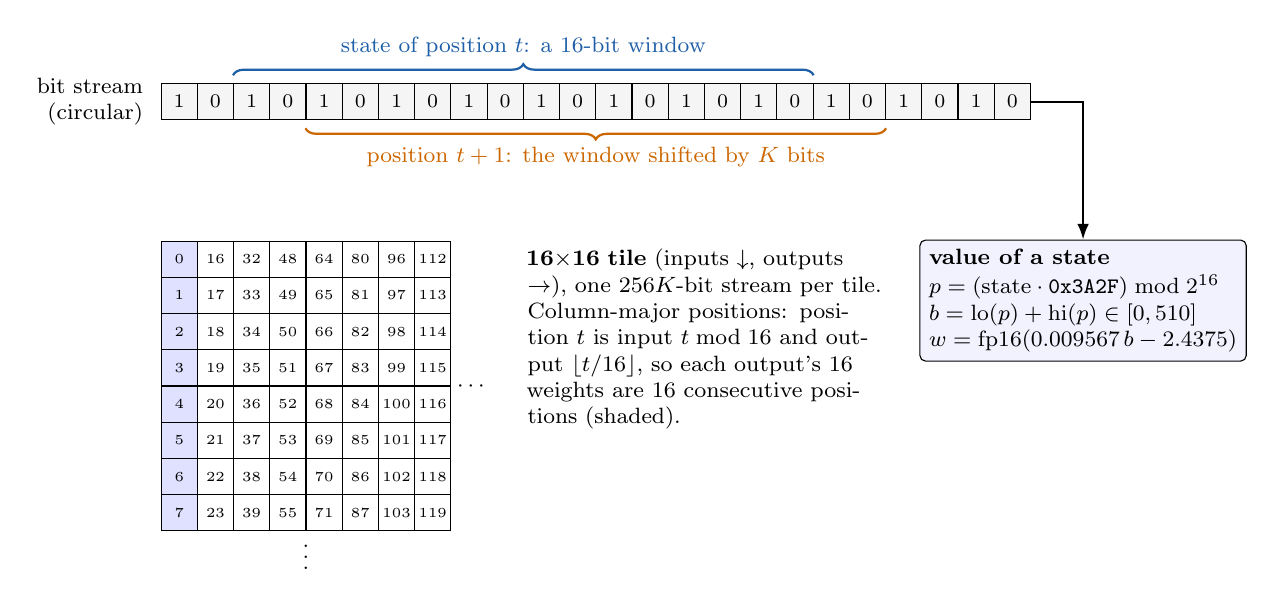
\begin{tikzpicture}[font=\footnotesize, cell/.style={draw, minimum size=4.6mm, inner sep=0}]
\foreach \i in {0,...,23} { \node[cell, fill=gray!8] (b\i) at (\i*0.46, 0) {}; }
\foreach \i in {0,...,23} { \pgfmathtruncatemacro{\v}{mod(\i*7+3,2)}; \node[font=\scriptsize] at (b\i) {\v}; }
\node[left=1mm of b0, align=right] {bit stream\\(circular)};
\draw[decorate, decoration={brace, amplitude=4pt}, thick, tsix] ($(b2.north west)+(0,0.1)$) -- node[above=3pt]{state of position $t$: a 16-bit window} ($(b17.north east)+(0,0.1)$);
\draw[decorate, decoration={brace, amplitude=4pt, mirror}, thick, orange!80!black] ($(b4.south west)+(0,-0.1)$) -- node[below=3pt]{position $t+1$: the window shifted by $K$ bits} ($(b19.south east)+(0,-0.1)$);
\begin{scope}[shift={(0,-2.0)}]
\fill[blue!12] (-0.23, 0.23) rectangle (0.23, -7*0.46-0.23);
\foreach \c in {0,...,7} { \foreach \r in {0,...,7} {
  \pgfmathtruncatemacro{\t}{\c*16+\r}
  \node[cell] at (\c*0.46, -\r*0.46) {\tiny \t};
}}
\node at (8*0.46+0.05, -3.5*0.46) {$\cdots$};
\node at (3.5*0.46, -8*0.46) {$\vdots$};
\node[align=left, anchor=north west, text width=46mm] at (4.3, 0.25) {\textbf{16$\times$16 tile} (inputs $\downarrow$, outputs $\rightarrow$), one $256K$-bit stream per tile. Column-major positions: position $t$ is input $t \bmod 16$ and output $\lfloor t/16 \rfloor$, so each output's 16 weights are 16 consecutive positions (shaded).};
\node[draw, rounded corners=2pt, fill=blue!5, align=left, anchor=north west] (f) at (9.4, 0.25) {\textbf{value of a state}\\[1pt]$p = (\text{state}\cdot \texttt{0x3A2F}) \bmod 2^{16}$\\$b = \text{lo}(p) + \text{hi}(p) \in [0, 510]$\\$w = \mathrm{fp16}(0.009567\,b - 2.4375)$};
\end{scope}
\draw[-{Latex[length=2mm]}, thick] (b23.east) -| (f.north);
\end{tikzpicture}
\caption{T16's storage. Each weight's state is a 16-bit window of its tile's circular bit stream. Consecutive
positions overlap by $16-K$ bits, so a weight costs $K$ bits; at half-integer $K$, even and odd positions alternate
$\lfloor K \rfloor$ and $\lfloor K \rfloor + 1$ bits. The value is a two-byte sum of a 16-bit product (top right).
Positions are column-major inside the tile (bottom).}
\label{fig:trellis}
\end{figure}

T16 is EXL3's storage format with a different value function and position order (\cref{fig:trellis}). An expert
matrix $W$ ($k$ inputs, $n$ outputs) computes
\begin{equation}
y = s_v \odot \mathcal{H}_{128}\big(\mathcal{H}_{128}(x \odot s_u)\, W_{\text{inner}}\big),
\end{equation}
where $\mathcal{H}_{128}$ is the orthonormal Walsh-Hadamard transform over blocks of 128, $s_u \in \mathbb{R}^k$ and
$s_v \in \mathbb{R}^n$ are per-channel scales (fp16), and $W_{\text{inner}}$ is stored as 16$\times$16 tiles. Each
tile is one circular bit stream of $256K$ bits, decoded at $L = 16$.

\paragraph{The codebook.}
A state $s$ maps to $p = (s \cdot \texttt{0x3A2F}) \bmod 2^{16}$, $b = (p \mathbin{\&} \texttt{0xFF}) + (p \gg 8)$, and
$w = \mathrm{fp16}(\mathrm{fma}(1024 + b,\ \texttt{0x20e6},\ \texttt{0xca1e}))$. That is $0.009567\,b - 2.4375$
rounded to fp16, one of 511 values, approximately Gaussian because $b$ sums two roughly uniform bytes. On the CPU,
\texttt{vpmullw} multiplies 16 windows in one instruction (against 8 for \texttt{vpmulld}, at twice the throughput), and
\texttt{vpdpbusd} takes the two bytes against the activations, two weights per 32-bit lane (\cref{eq:fused}). We searched
the multiplier, byte-sum width and table-based alternatives with Viterbi on i.i.d.\ Gaussian tiles (\cref{fig:mse}).
T16's MSE is 0.0665 against \texttt{mul1}'s 0.0640 at 2 bits, a 4\% increase worth about 0.03 bits per weight. The
constant matters: \texttt{0xD12D} is 11\% worse. Shuffle-only nibble tables are 21\% worse.

\begin{figure}[t]
\centering
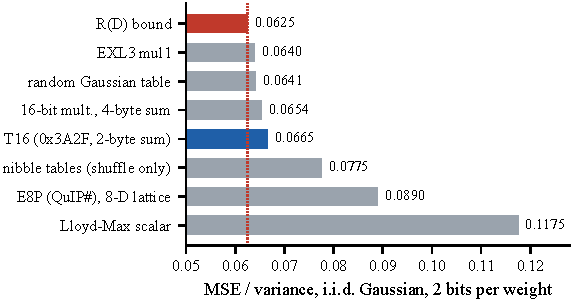
\includegraphics[width=0.48\linewidth]{figs/codebook_mse.pdf}\hfill
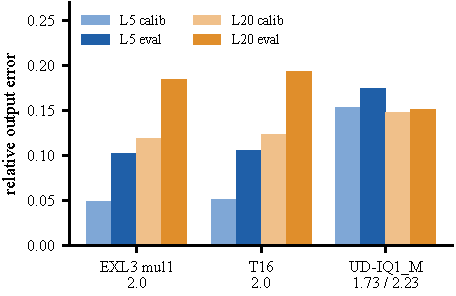
\includegraphics[width=0.48\linewidth]{figs/transfer.pdf}
\caption{Left: codebook accuracy at 2 bits on i.i.d.\ Gaussian tiles (Viterbi at the best scale; E8P from
QTIP~\cite{qtip}). Right: relative output error of real V4.1 experts (every 8th expert of layers 5 and 20) on
calibration tokens and on held-out evaluation tokens, with the full input Hessian. T16 stays within 4\% of
\texttt{mul1}. Both trellis codes lose 1.6--2.4$\times$ from calibration to new text, while UD-IQ1\_M's experts lose
1.0--1.2$\times$; this is the transfer gap that \cref{sec:quantizer,sec:calib} address.}
\label{fig:mse}
\end{figure}

\paragraph{Column-major positions.}
EXL3 orders a tile's 256 positions in the fragment order of the \texttt{mma.m16n8k16} tensor-core instruction, which
suits batched GEMMs. For single-token GEMVs we want each output's 16 weights in 16 consecutive positions, so that a
lane walks one output column with plain window shifts. Because LDLQ quantizes 16-row bands and the Viterbi search sees a
256-weight sequence of near-Gaussian values after the Hadamard transforms, the order should not matter for quality.
\Cref{tab:order} confirms it: with only ExLlamaV3's permutation swapped, calibration error agrees within 0.3\%, and the
evaluation ratios ($+2.7\%$, $-1.3\%$) are per-expert noise, with medians of 1.00.

\begin{table}[t]
\centering\small
\begin{tabular}{@{}llrrrl@{}}
\toprule
Layer, $K$ (gate/up/down) & Tokens & Tensor-core order & Column-major & Ratio & Per expert \\
\midrule
5, 1.5/1.5/2 & calibration & 0.07943 & 0.07966 & 1.003 & 0.98--1.01 \\
5, 1.5/1.5/2 & evaluation & 0.12765 & 0.13111 & 1.027 & median 1.005 \\
20, 2/2/2.5 & calibration & 0.06726 & 0.06719 & 0.999 & 0.99--1.01 \\
20, 2/2/2.5 & evaluation & 0.09808 & 0.09678 & 0.987 & median 1.000 \\
\bottomrule
\end{tabular}
\caption{Tile position order does not affect quality. Relative output error, $\sum \lVert \hat y - y\rVert^2 / \sum
\lVert y\rVert^2$ over 12 experts per layer, damped Hessian ($\sigma_{\text{reg}} = 2$). Gaussian tiles: 0.07122 vs
0.07124.}
\label{tab:order}
\end{table}

\paragraph{Kernels.}
The GPU kernel gives each lane one output column of a tile pair and walks down the inputs. A running pointer and one
16-byte activation load serve 8 rows; the windows of a column come from one 64-bit view of the stream; and two rows'
products are packed per \texttt{dp4a} with int8 activations (one scale per 256 inputs). SASS shows 1.66 ALU and 1.72
FMA-heavy instructions per weight, against the model's 1.5 + 1.5. The kernel is bound by load latency rather than by
decode math. On the CPU, the column views come from byte-aligned 16-byte loads and one \texttt{vpshufb} per four
columns (tile words byte-swapped once at load), then one shift, one \texttt{vpmullw} and one \texttt{vpdpbusd} per
weight class. \Cref{fig:decode} compares both with dsx's kernels for the IQ formats of UD's mix, measured interleaved in
one session. At 2 bits T16 takes 29--31\% less GPU time than IQ2\_XXS and faster than every IQ format at every rate,
plus $\sim$6\,$\mu$s per call for its two Hadamard transforms and scales, which can be fused into the activation
kernels that run anyway. On the CPU T16
beats the UD mix at 1.5 and 2 bits, and at 2.5 bits it is within 3\% and bound by RAM.

\begin{figure}[t]
\centering
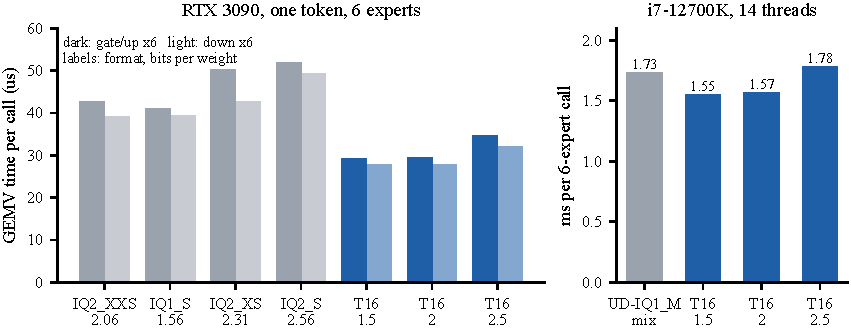
\includegraphics[width=\linewidth]{figs/decode_cost.pdf}
\caption{Decode cost per call of 6 experts (one token), measured on the target machine. Left: RTX 3090 GEMV, nsys
medians at 285\,W over two interleaved rounds; IQ tiles are dsx's kernels for ggml's formats. Right: i7-12700K, 14
threads, interleaved with UD-IQ1\_M's layer mix.}
\label{fig:decode}
\end{figure}

\section{The quantizer}
\label{sec:quantizer}

We use ExLlamaV3's quantizer~\cite{exllamav3} (v1.6.4), patched for T16. Its \texttt{mul1} constants become T16's, its
tile permutation becomes column-major, and the Hessian stays on the GPU. For each expert matrix it rotates $W$ and the
input Hessian $H$ with randomized 128-wide Hadamard transforms, runs LDLQ over 16-row bands with a Viterbi search per
16$\times$16 tile (65{,}536 states, two passes for tail-biting), and refits the per-channel scales against $H$. The
Hessians come from a calibration chain that runs DeepSeek's reference model one layer at a time over the calibration
set and records every expert's routed inputs.

\paragraph{Damping.}
With the full Hessian, T16 experts fit their calibration tokens closely but lose 1.6--2.4$\times$ of their accuracy on
new text (\cref{fig:mse}, right). Each expert sees only the few thousand tokens routed to it, so its Hessian is a noisy
estimate. We regularize LDLQ with $\sigma_{\text{reg}} = 2$ (twice the mean diagonal), which keeps the fit general.

\paragraph{A dense fractional-rate Viterbi kernel.}
Half-integer rates, where positions alternate $\lfloor K \rfloor$ and $\lfloor K \rfloor{+}1$ bits, use a generic
kernel in ExLlamaV3. That kernel keeps its path costs in global memory, re-decodes all 65{,}536 codebook values at
every step, and stores a 16-bit predecessor per node at the widest stride (16\,MB of traceback per tile). ncu showed
it memory-bound: DRAM 68\% busy, one instruction per cycle, and no eligible warp in 73\% of cycles. We rebuilt it in
the style of ExLlamaV3's dense integer-rate kernels. Each of 1024 threads owns the same 64 states at every step,
whatever the step's width, so the decoded values stay in registers. The costs live in shared memory, one buffer per
node width, and with alternating widths a step reads one buffer and writes the other, so it needs one barrier. The
history stores each node's chosen branch, packed by warp ballots into 1\,MB per tile. Arithmetic and tie order are
unchanged, so the indices are bit-identical: we verified this on Gaussian tiles and on every tensor of three real
experts. The new kernel is bound by the shared-memory pipe (79\%, 2.5 instructions per cycle).
\Cref{fig:viterbi} shows the effect: 5.1$\times$ at 1.5 bits, 2.1$\times$ at 2.5 bits, and per-expert time
16.3\,s $\to$ 5.0\,s at the 1.5-bit layout. That cut the full-model quantization estimate from $\sim$50 to $\sim$23
RTX 3090-hours.

\begin{figure}[t]
\centering
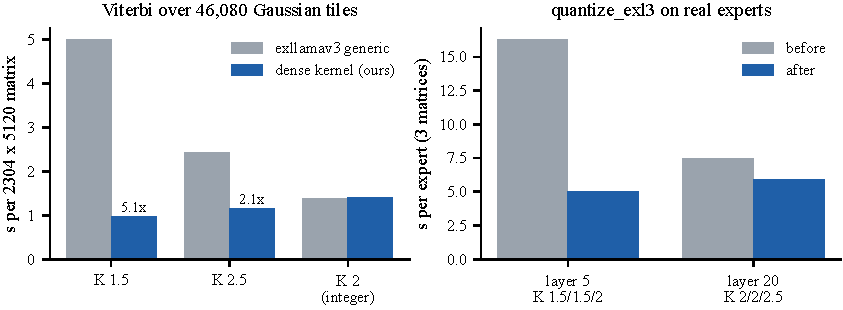
\includegraphics[width=\linewidth]{figs/viterbi.pdf}
\caption{The dense fractional-rate Viterbi kernel (RTX 3090 at 250\,W). Left: one $2304 \times 5120$ matrix of
Gaussian tiles, ExLlamaV3's generic kernel against ours, with identical indices; the integer-rate kernel at $K=2$ is
shown for reference. Right: \texttt{quantize\_exl3} per expert on real V4.1 experts.}
\label{fig:viterbi}
\end{figure}

\subsection{Output shrinkage and a free gain correction}
\label{sec:gain}

A reconstruction that minimizes squared error is biased toward zero. If $Q$ is the MSE-optimal reconstruction of $W$
from its code, the error is orthogonal to it, $\langle W - Q, Q\rangle = 0$, so the gain is
\begin{equation}
g \;=\; \frac{\langle Q, W\rangle}{\langle W, W\rangle} \;=\; \frac{\lVert Q\rVert^2}{\lVert W\rVert^2} \;=\; 1 - \frac{\lVert W - Q\rVert^2}{\lVert W\rVert^2}.
\end{equation}
The Viterbi search with a refit scale behaves like this. On a layer-5 expert, the relative weight error is 0.151 at 1.5
bits and 0.075 at 2 bits, and the measured gains are 0.862 and 0.929, close to $1 - $ the error (0.849 and 0.925). Per matrix, shrinking is the right choice, since
it cuts noise more than it adds bias. In a network, however, the bias is the same sign in every expert of every layer,
and it compounds through 40 residual blocks.

We correct it in the stored output scales $s_v$, which costs nothing at run time. Sweeping the gain on a model with T16
experts in layers 0--19 (1.5-bit gate/up) took KL from 0.3145 to 0.2503 at $\times 1.13$ (\cref{fig:gain}, left).
On the full model, the 2-bit gate/up optimum is $\times 1.04$ (KL 0.1962 $\to$ 0.1943, right). Down projections did not
benefit. The KL-optimal factors sit between the plain gain and the gain weighted by the input Hessian, which is
0.96--0.97 on calibration activations. We read this as one more symptom of the calibration-to-evaluation transfer gap:
on held-out activations the shrinkage is larger than the calibration Hessian suggests. The factors were chosen on the
evaluation set itself, which we note as a limitation (\cref{sec:limits}). From now on, the worker records both gains
for every matrix, so that per-expert corrections can later be fit on held-out activations.

\begin{figure}[t]
\centering
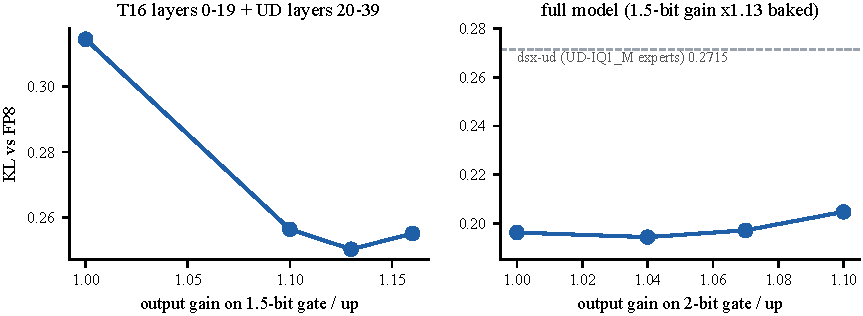
\includegraphics[width=\linewidth]{figs/gain.pdf}
\caption{Output-gain sweeps (Lucebox KL vs FP8). Left: T16 experts in layers 0--19 (UD's elsewhere), gain on 1.5-bit
gate/up. Right: full T16 model with $\times 1.13$ baked in, gain on 2-bit gate/up; dsx-ud for reference.}
\label{fig:gain}
\end{figure}

\section{Calibration for a 384-expert MoE}
\label{sec:calib}

Each expert's Hessian is built from the tokens routed to it, so calibration has to cover the experts as well as the
domains. The first full run (calib4) used 715K tokens, of which 635K fed the Hessians. It combined coding-agent
sessions, agent and code prompts, the model's own reasoning traces, Wikipedia in five languages, the-stack-smol code
and UltraChat.

\paragraph{calib5.}
An audit of calib4 found 37K tokens of web text, agent sequences that are mostly prompts and tool output (11K
assistant tokens out of 103K), Wikipedia drawn only from alphabetically early articles, and 80K tokens held out for a
screening step the trellis pipeline does not use. calib5 drops the web text and uses every sequence for the Hessians.
It adds three sources:
\begin{itemize}\setlength{\itemsep}{1pt}
\item 253K tokens of real coding-agent transcripts, scrubbed of credentials before they left the machine that held
them (presigned URLs, environment-style secrets, keys and tokens, emails; checked with an independent scan) and
rendered with DeepSeek's V4.1 chat encoder, with tool calls and thinking blocks;
\item SWE-smith agent trajectories~\cite{swesmith}, converted to the model's tool-call format;
\item R1-0528 reasoning traces~\cite{amr1}.
\end{itemize}
It also samples Wikipedia at random from ten languages and keeps the model's own reasoning traces. Every text is
filtered against the evaluation set with 50-character shingles. Every rendered window fits one 2048-token row.

\paragraph{Coverage top-up.}
A routing-only pass over the base set plus a 428K-token candidate pool counts each (layer, expert)'s tokens. A greedy
selector then adds the pool rows that fill the most remaining deficit below 256 tokens, under a cap that keeps the set
at or below 1.25M tokens. The rarest expert in calib4 (layer 22, expert 310, 12 tokens) fired on the concept of
dividing (the character \emph{f\=en} and ``divided into''), almost only in Chinese and Japanese Wikipedia, so the pool was weighted toward those languages and code. The selector added 69 rows, giving 1{,}177{,}600
tokens. It reduced the experts below 256 tokens from 24 to 8 and raised the worst per-layer minimum from 60 to 91
(\cref{fig:coverage}). It stopped before its cap because the pool held nothing for the last 8 experts; those need
targeted text. On the Lucebox evaluation the calib5 model scores KL 0.202 against calib4's 0.196, with slightly higher
top-1 agreement (81.3\% vs 80.9\%). Two caveats apply. The output gains were tuned on the calib4 model and reused
unchanged. And calib5 removed the web text that calib4 contained, which is the closest domain to this evaluation's
text. calib5 was built for agentic use, which this evaluation does not measure, so we report it as an open result.

\begin{figure}[t]
\centering
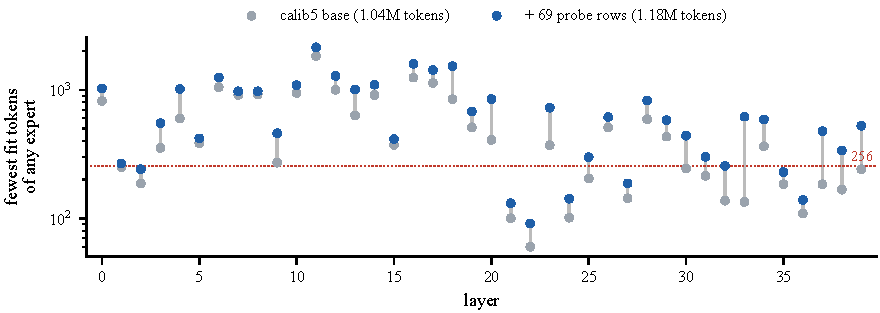
\includegraphics[width=\linewidth]{figs/coverage.pdf}
\caption{Fewest calibration tokens of any expert, per layer, before and after the probe top-up (calib5). The probes
were mostly agent trajectories (28 rows), code (15), reasoning (13) and Chinese and Japanese Wikipedia (6).}
\label{fig:coverage}
\end{figure}

\section{Results}
\label{sec:results}

\paragraph{Setup.}
Experts use 1.5/1.5/2 bits (gate/up/down) in layers 0--19 and 2/2/2.5 in layers 20--39, about 1.9 bits per weight,
sized to match UD-IQ1\_M. The 15{,}360 experts take 131\,GB. Dense weights are Q8\_0, and the Engram table is IQ4\_NL
(or Q6\_K). The whole model ships as one GGUF file with the tokenizer inside~\cite{dsxt16}. Quality is measured on the
Lucebox evaluation set~\cite{lucebox}: 8$\times$1024 tokens scored against the FP8 model's top-256 log-probabilities
(KL divergence, top-1 agreement, perplexity). Speed is measured on 2$\times$RTX 3090 (250/280\,W), an i7-12700K and
128\,GB of DDR4.

\begin{table}[t]
\centering\small
\begin{tabular}{@{}lllrrrr@{}}
\toprule
Build & Experts & Runtime & GB & KL $\downarrow$ & Top-1 $\uparrow$ & PPL $\downarrow$ \\
\midrule
FP8 (reference) & FP4 / FP8 & & & 0 & 100\% & 8.56 \\
dsx-2bit v4b & scalar ternary / 2 / 3-bit & dsx & 148 & 0.373 & 74.4\% & 10.68 \\
Unsloth UD-IQ1\_M & IQ1\_S/IQ2\_* mix & llama.cpp & $\sim$140 & 0.275 & 78.8\% & 10.11 \\
dsx-ud & UD-IQ1\_M's experts & dsx & 142 & 0.272 & 79.0\% & 10.17 \\
Maya-S & llama.cpp mix & llama.cpp & 178 & 0.195 & 82.0\% & 9.49 \\
\textbf{dsx-t16 v1} (IQ4\_NL Engram) & \textbf{T16} & dsx & \textbf{141} & \textbf{0.196} & \textbf{80.9\%} & \textbf{9.54} \\
\textbf{dsx-t16 v1} (Q6\_K Engram) & \textbf{T16} & dsx & \textbf{141} & \textbf{0.194} & \textbf{81.4\%} & \textbf{9.60} \\
dsx-t16 v2, calib5 (IQ4\_NL Engram) & T16 & dsx & 141 & 0.202 & 81.3\% & 9.58 \\
\midrule
\multicolumn{7}{@{}l}{\emph{Decode path (one token at a time, 2{,}046 tokens)}} \\
dsx-ud & & dsx & 142 & 0.303 & 80.4\% & 9.03 \\
\textbf{dsx-t16 v1} & & dsx & \textbf{141} & \textbf{0.205} & \textbf{82.0\%} & \textbf{8.65} \\
\bottomrule
\end{tabular}
\caption{Quality against the FP8 model (Lucebox 1017 evaluation). GB counts experts and dense weights, without the
Engram table. T16 v1 uses calib4, v2 calib5 with v1's output gains; v1 and v2 were measured in one session.}
\label{tab:quality}
\end{table}

\paragraph{Quality.}
\Cref{tab:quality,fig:pareto} summarize quality. At the same size as dsx-ud, T16's experts lower KL by 28\%
(0.272 $\to$ 0.194) and raise top-1 agreement from 79.0\% to 81.4\%. That is about the quality of the 178\,GB Maya-S
build in 141\,GB. Through the decode path, the gap is the same (0.303 $\to$ 0.205). Relative to dsx's earlier scalar
formats at 148\,GB, KL drops by 48\%. The gain correction is essential: without it, T16 experts in layers 0--19 made the model worse than UD's experts
there (KL 0.3145 against dsx-ud's 0.2715), and with it they made it better (0.2503).

\begin{figure}[t]
\centering
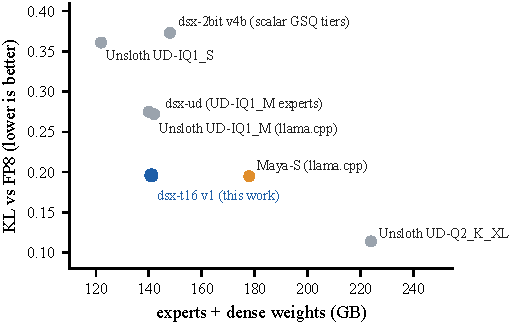
\includegraphics[width=0.52\linewidth]{figs/pareto.pdf}
\caption{Quality per byte on the Lucebox evaluation (KL vs FP8, experts and dense weights without the Engram table).}
\label{fig:pareto}
\end{figure}

\paragraph{Speed.}
On the same machine, with dsx-ud measured in the same session (\cref{tab:speed}), T16 decodes the same 2{,}046
teacher-forced tokens 15\% faster (215\,s vs 253\,s). Free-running decode after a 3K-token prompt reaches 34.9 tokens/s
against 27.9--28.0. Per layer, T16's experts compute 20--34\% faster on the CPU (1.21/1.46\,ms per 6-expert call vs
1.83, 14 threads) and 22\% faster on the GPU (125 vs 161\,$\mu$s). Prefill is 9\% slower for now. An nsys profile of
a 3K-token prefill shows the first T16 dequantize-to-fp16 kernel taking 3.6\,s of GPU0's 6.6\,s of kernel time (127
$\mu$s per call). A rewritten kernel is 2.5--3.0$\times$ faster on an RTX 3090 and bit-identical. In the same session it raises
3K-token prefill from 388 to 415--428 tokens/s, closing most of the gap to dsx-ud.

\begin{table}[t]
\centering\small
\begin{tabular}{@{}lrr@{}}
\toprule
2$\times$RTX 3090 + i7-12700K + 128 GB & dsx-t16 & dsx-ud \\
\midrule
Decode, the same 2{,}046 tokens (teacher-forced) & \textbf{215 s} & 253 s \\
Decode, 3K-token prompt + 300 tokens & \textbf{34.9 tok/s} & 27.9--28.0 tok/s \\
Decode with expert deferral (\texttt{--defer-rank 3}) & \textbf{36.8 tok/s} & 36.1--36.2 tok/s \\
Prefill, 3K-token prompt & 361--367 tok/s & 393--409 tok/s \\
Expert compute per layer, CPU (6 experts, 14 threads) & \textbf{1.21 / 1.46 ms} & 1.83 ms \\
Expert compute per layer, GPU (6 resident experts) & \textbf{125 $\mu$s} & 161 $\mu$s \\
\bottomrule
\end{tabular}
\caption{Speed. Free-running decode generates different text per build, which moves the share of experts the CPU
computes; the teacher-forced row is the like-for-like comparison.}
\label{tab:speed}
\end{table}

\paragraph{Quantization cost.}
The first full run quantized all 15{,}360 experts on one rented RTX PRO 6000 (96\,GB) in 6.1 hours. The calibration
chain ran alongside two quantization workers under NVIDIA MPS (2.45--2.6\,s per expert each), and layers were uploaded
as they finished, at \$2.61/h for \$16.00, plus \$0.65 for rentals that failed a network check. A third worker added no
throughput. The calib5 requant split the layers into two blocks on two pods, each running the chain from layer 0 to
its block's end. It took 6.3 hours of wall time and \$33.20; the larger calibration set raised the time per expert to
2.9--3.0\,s.

\section{Packaging}
T16 ships inside GGUF as dsx-specific tensor types (ids 1010--1012, one per rate), so the model, tokenizer and
metadata stay in one file set. Hugging Face's GGUF parser accepts the unknown ids and counts parameters from the
shapes; llama.cpp's tools reject them. We decided against an EXL3-layout export. ExLlamaV3 identifies its codebook by
the presence of a \texttt{mul1} tensor and assumes tensor-core position order, so it would load T16 files and silently
produce wrong weights. A byte-exact specification (\cref{app:spec}) and a NumPy reference decoder, which reproduces
ExLlamaV3's reconstruction bit for bit on golden files, document the format.

\section{Limitations}
\label{sec:limits}
\begin{itemize}\setlength{\itemsep}{1pt}
\item The output gains ($\times 1.13$, $\times 1.04$) were chosen on the evaluation set used for the results, so the
reported KL is slightly optimistic. Fitting per-expert gains on held-out activations is future work.
\item All quality numbers come from one evaluation set of 8$\times$1024 tokens. We did not run downstream task suites.
\item Trellis experts still transfer from calibration to new text worse than UD's codebook experts per unit of
calibration error. Damping and broader calibration narrow the gap; YAQA-style~\cite{yaqa} Hessians or fine-tuning
might close it, but at a cost beyond our budget.
\item T16 is specific to dsx. It is not loadable by ExLlamaV3 or llama.cpp, and quantization needs a GPU because the
Viterbi search runs over 65{,}536 states.
\item The broader calibration set (calib5) did not lower KL on this evaluation (0.202 vs 0.196) with reused gains.
Whether it helps agentic workloads, as intended, needs an evaluation on such text.
\end{itemize}

\section{Conclusion}
For a 552B MoE on a desktop, the expert format is a systems problem: it has to decode at memory speed on two kinds of
processor. Designing the codebook from a measured instruction budget gives T16, which costs 4\% more MSE than
ExLlamaV3's codebook on Gaussian data but decodes faster than every IQ format on both the GPU and the CPU. Combined
with ExLlamaV3's quantizer, a damped Hessian, a free output-gain correction and routing-aware calibration, it lowers KL
by 28\% at equal size and speeds up decode, on hardware that costs less than a single datacenter GPU.

\paragraph{Acknowledgments.}
We thank DeepSeek for releasing the model, turboderp for ExLlamaV3, the QTIP authors for bitshift trellises, the
llama.cpp and Unsloth teams for their formats and builds, Lucebox for the evaluation set, and the Xolotl/Strata
contributors for the V4.1 GGUF tooling. This work was carried out with several Claude Code (Anthropic) agent sessions
working under the author's direction.

\bibliographystyle{plainnat}
\bibliography{refs}

\appendix
\section{T16 format specification}
\label{app:spec}
An expert matrix with $k$ inputs and $n$ outputs ($k, n$ multiples of 128) is stored as:
\begin{itemize}\setlength{\itemsep}{1pt}
\item \textbf{Tiles.} Tile $(k_b, n_b)$ covers inputs $16k_b \ldots 16k_b{+}15$ and outputs $16n_b \ldots 16n_b{+}15$.
Tiles are stored by tile column (index $n_b \cdot k/16 + k_b$), $32K$ bytes each (48/64/80 bytes at 1.5/2/2.5 bits).
\item \textbf{Bit stream.} Each tile is one circular stream of $256K$ bits; byte 0 holds bits 0--7, most significant bit
first.
\item \textbf{Positions.} Position $t$ is input $t \bmod 16$ and output $\lfloor t/16\rfloor$. At integer $K$, position
$t$'s bits end at $(t+1)K$. At half-integer $K$, even positions take $\lfloor K\rfloor$ bits and odd positions one
more, ending at $(t+1)\lfloor K\rfloor + \lfloor (t+1)/2\rfloor$.
\item \textbf{State and value.} The state is the 16 bits ending at the position's end bit, MSB first, wrapping around
the stream. $p = (\text{state}\cdot \texttt{0x3A2F}) \bmod 2^{16}$, $b = (p \mathbin{\&} \texttt{0xFF}) + (p \gg 8)$,
and the value is $\mathrm{fp16}(\mathrm{fma}(\mathrm{fp16}(1024+b), \mathrm{fp16}\ \texttt{0x20e6}, \mathrm{fp16}\
\texttt{0xca1e}))$: the exact product and sum, rounded once.
\item \textbf{Scales and transforms.} $s_u$ (fp16, $[k]$) and $s_v$ (fp16, $[n]$);
$y = s_v \odot \mathcal{H}_{128}(\mathcal{H}_{128}(x \odot s_u)\, W_{\text{inner}})$ with orthonormal Walsh-Hadamard
blocks of 128. Output gains, where used, are already multiplied into $s_v$.
\end{itemize}
ExLlamaV3's own layout is \texttt{int16 [k/16][n/16][16K]}, read as little-endian 32-bit words, MSB first. The dsx
layout reorders the tiles by column and byte-swaps each 32-bit word. The reference code is
\nolinkurl{core/src/t16.rs}, \nolinkurl{quant/t16/t16_ref.py} and \nolinkurl{docs/t16-format.md} in the dsx
repository~\cite{dsx}.

\end{document}
